El método implementado utiliza el concepto de la distancia de Levenshtein\footnote{La distancia de Levenshtein corresponde a la cantidad de cambios necesarios en un string para transformarlo en un string objetivo.} para determinar si el texto proporcionado por el usuario como ubicación corresponde o no a una comuna existente en Chile. La información relativa a las actuales comunas, provincias y regiones de acuerdo al Decreto Exento Nº 817, del Ministerio del Interior, publicado en el Diario Oficial del 26 de Marzo de 2010 \cite{listaCodigosProvincias}. La posición GPS de cada una de las provincias se obtuvo mediante la ubicación proporcionada en \cite{dicesmapas}.

\begin{algorithm}
	\caption{Reconocimiento de ubicación del usuario mediante Levenshtein}\label{ciudadesLeven2}
	\begin{algorithmic}[1]
		\Function{getDistanciaLeven}{usuarios}
		\For{usuario in usuarios}
		\State usuario.ubicacion = limpiarPuntuacion(usuario.ubicacion)\;
		\State usuario.ubicacion = quitarNacionalidad(usuario.ubicacion)\;
		\For{comuna in comunas}
		\State dist = Levenshtein(comuna, usuario.ubicacion)\;
		\If{dist\textless MinimaDistancia}
		\State usuario.comuna = comuna\;
		\EndIf
		\EndFor
		\EndFor
		\EndFunction
	\end{algorithmic}
\end{algorithm}

%\begin{algorithm}
%	\caption{Reconocimiento de ubicación del usuario mediante SQL}\label{ciudadesSql}
%	\begin{algorithmic}[1]
%		\For{comuna in comunas}
%			\State usuariosComuna = getUsersFromBd(comuna)
%			\For{usuario in usuariosComuna}
%				\State usuario.comuna = comuna
%			\EndFor
%		\EndFor	
%	\Function{getUsersFromBd}{comuna}
%		\State sql = 'SELECT usuario WHERE usuario.ubicacion LIKE "\%" + comuna;
%		\State return execute(sql);
%	\EndFunction	
%	\end{algorithmic}
%\end{algorithm}

\subsubsection{Prueba valores distancia Levenshtein para identificar ubicación}

Para obtener cual es la distancia de Levenshtein con mejores resultados se consideró una muestra representativa de 383 usuarios elegidos de manera aleatoria y cuyo campo ubicación fuese distinto a vacío.

Los resultados obtenidos fueron los siguientes:

\begin{table}[H]
	\centering
	\begin{tabular}{| c|c|c|c|}
		\hline
		D. Levenshtein & Nº match correctos & Nº match incorrectos  &  Error porcentual \\ \hline
		1   & 157 & 157 & 0,00\% \\ \hline
		2   & 172 & 164 & 2,09\% \\ \hline
		3	& 207 & 189 & 4,70\% \\ \hline
		4	& 223 & 192 & 8,09\% \\ \hline
		5	& 235 & 194 & 10,70\% \\ \hline
	\end{tabular}
	\caption {Tabla comparativa para distintas valores de distancia de Levenshtein}
\end{table}

Podemos observar que a medida que aumentamos la distancia de Levenshtein, va aumentando la cantidad de coincidencias correctas pero también la cantidad de falsas coincidencias que ocurren.

Se consideró que un error menor al 5\% es adecuado, considerando la cantidad de coincidencias correctas que aporta al conjunto. Por lo anterior se concluye que la distancia de Levenshtein a utilizar corresponde a 3. Considerando este parámetro el número de coincidencias entre el campo ubicación y los nombre estándar de las comunas es de 114.016 del total de 650.000 usuarios (correspondiente al 17,54\% de usuarios). Éste porcentaje comparativamente es mayor que el 12\% encontrado por Cheng en \cite{Cheng:2010:YYT:1871437.1871535} mediante su primera metodología explicada en  \ref{sebsec:geoestadoarte}.

Al disponer los distintos usuarios en un mapa utilizando la API de mapas de Google, se obtienen la siguiente visualización:

\begin{figure}[H]
	\centering
	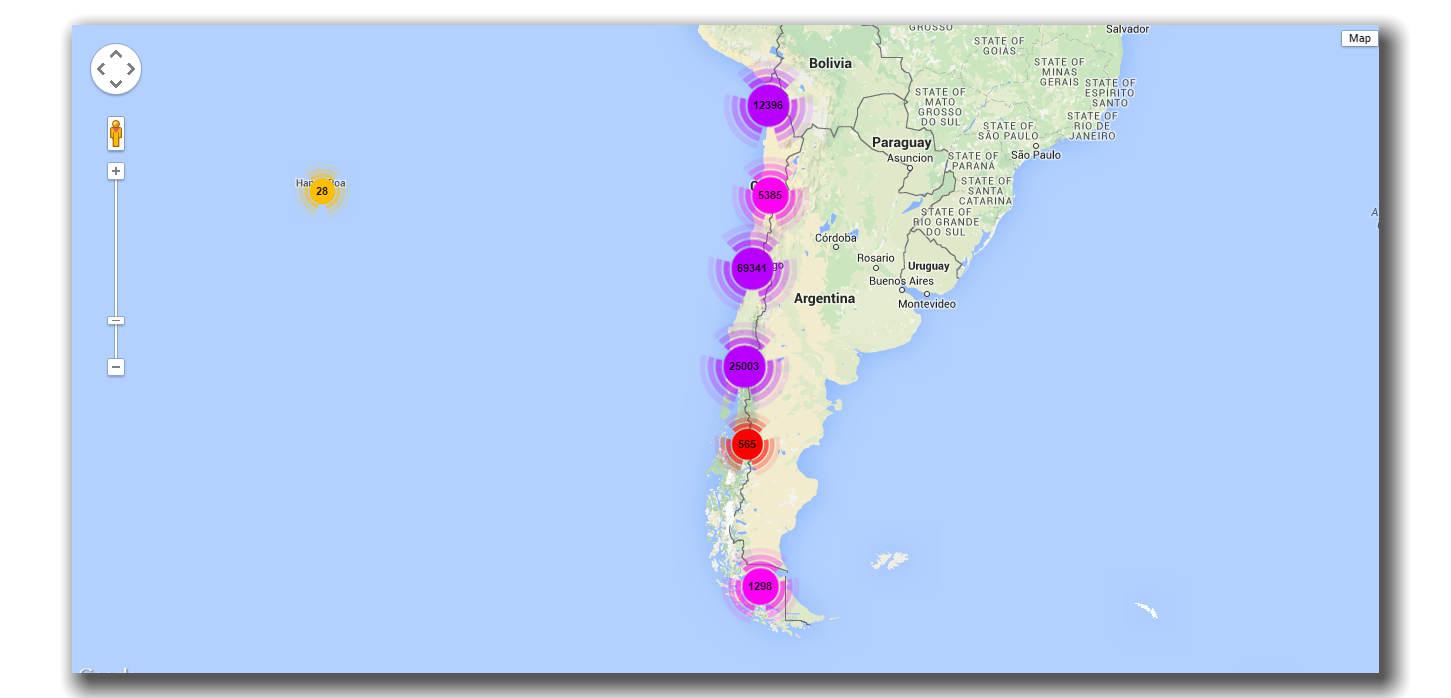
\includegraphics[width=0.9\textwidth]{imgs/mapa_usuarios.png}
	\caption{Mapa con los usuarios por ubicación geográfica}
	\label{fig:mapa_usuarios}
\end{figure}